To perform procedures, a project case has to be loaded first.
Each procedure will add a step to the project case.
For each procedure, there is an 'indicate' action when the user touches the trigger button, as well as an 'perform' action when the user presses the button.
This way, the user can touch the trigger button when he is about to perform a procedure and has visual feedback of when and where the procedure will start (i.e. tip of the surgical instrument).
Each time a procedure is performed, the user gets voice feedback that a step has been added.
The user can also navigate the steps by using voice commands, so that navigation thorugh the steps of the whole procedure can be done while holding surgical instruments.
At this point, six procedures are implemented in the system.
However, as described in Section \ref{sec::Architecture}, the system is extensible in the regard that new instruments can be implemented.
Currently, the implemented instruments are based on the workflow of OMF surgeons of the UHA: Users can perform drilling, hammer and chisel, bonesaw and milling operations.
Additionally, users can place markings and osteosynthesis plates on the virtual patient.
For some of the surgical instruments implemented, the user representation of the hand will be shown, for other not.
When a surgical instrument has this feature implemented, it is guaranteed that the instrument will always be grabbed and positioned as planned.
When this feature is missing, the user will not see his virtual hands on the surgical instrument, but can chose to hold it however he wants.
The decision, on which was decided if a surgical instrument should have this feature implemented, was made by a trial and error approach in which was investigated whether this feature was helpful or frustrating.

\paragraph{Drilling}

The \textbf{drilling} operation is performed by first picking up the drill handle from the instrument tray via the grabbing action (Figure \ref{fig::FeatureDrillingAttachments}).
Since drills are typically held in a number of different ways, the handgrip of the drill handle is adjustable.
Therefore, the virtual hand will not be displayed while holding the drill.
The instrument tray is located next to the operating table, where the patient's model will initially be positioned.
The drill handle initially has no attachment; users have to attach a drill bit first.

\begin{figure}[ht]
    \centering
    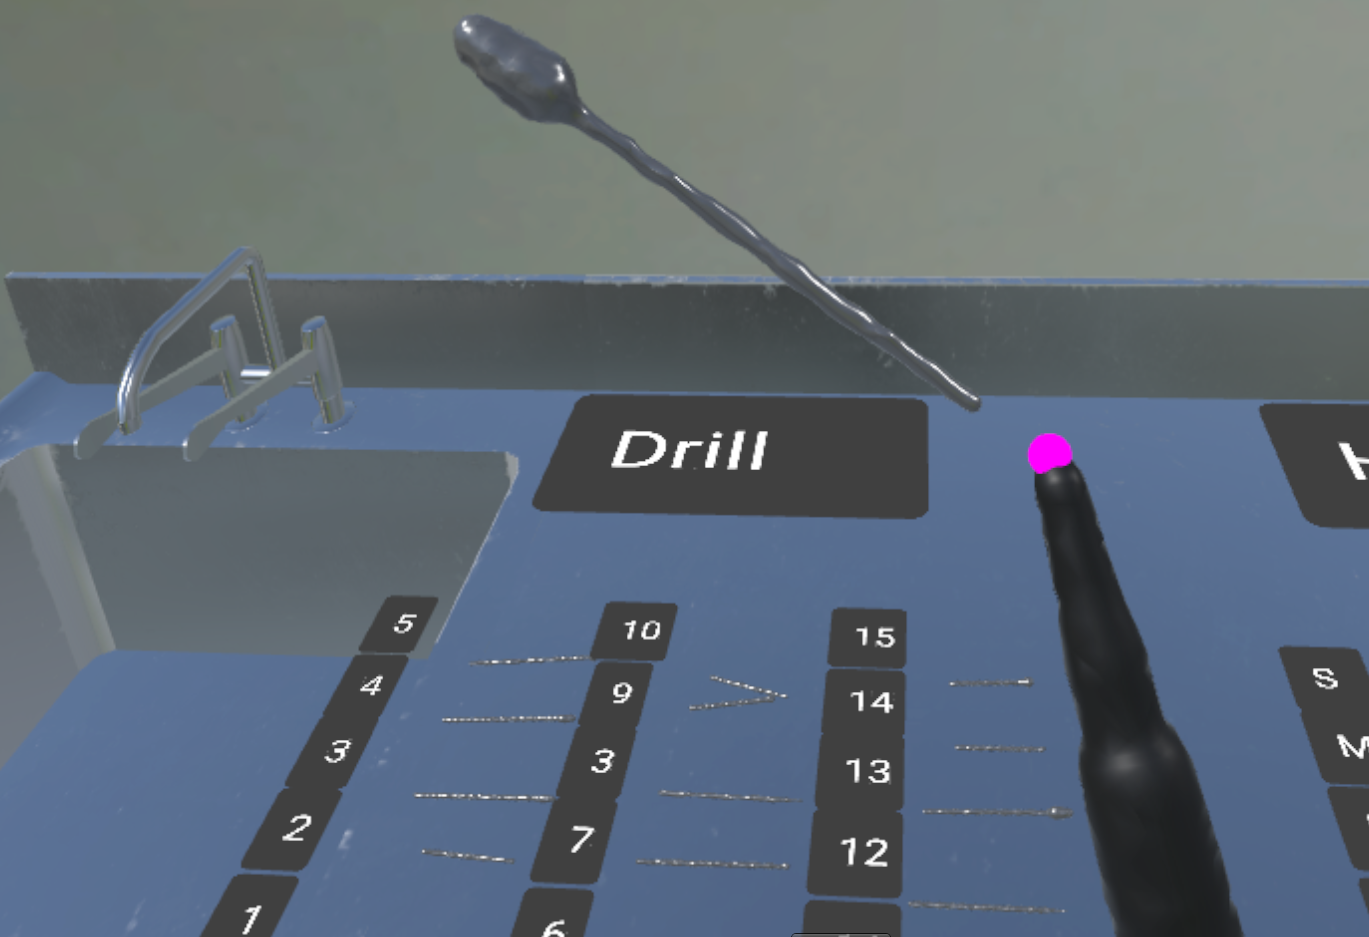
\includegraphics[width=200px]{images/implementation/features/procedures/drilling_attachment.png}
    \caption{\label{fig::FeatureDrillingAttachments}Process of attaching drill bit to the drill handle. With the right hand, the user performs the indicate action by touching 
    the respective button. With the other hand, the bit is picked up by grabbing it and moved into the pink sphere to attach the attachment.}
\end{figure}

In total, there are fifteen bits which can be used as an attachment for the drilling procedure.
Bits are modeled after their real counterparts in UHA.
They differ in size, length and width.
A visual signal is shown to the user while the indicate action is performed on the hand holding the drill handle.
By moving a drill bit to the visual indicator, the bit is attached to the handle (Figure \ref{fig::FeatureDrillingAttachments}).
Swapping out bits is performed by simply moving another bit into the indicator.
To perform the procedure, the drill handle must have a bit attached. 

\begin{figure}[ht]
    \centering
    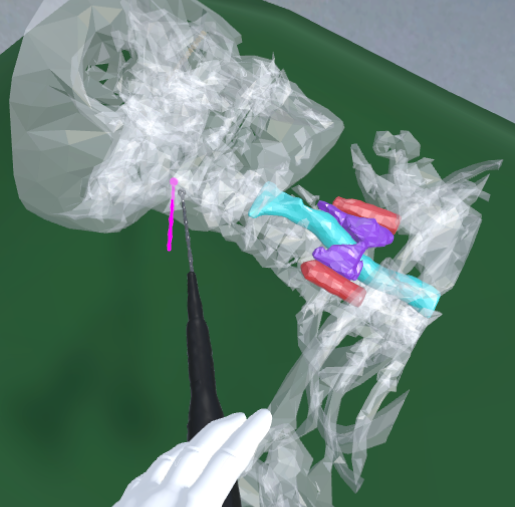
\includegraphics[width=200px]{images/implementation/features/procedures/drilling.png}
    \caption{\label{fig::FeatureDrilling}Drilling procedure. The pink object represents the last performed step, which was performed using the currently selected tool by pressing 
    the respective button all the way.}
\end{figure}

By triggering the perform action of the hand holding the drill, a copy of the currently attached drill bit is created and added to the project case. 
This copy has a different material, i.e. a pink material, to indicate that it is part of the project case (Figure \ref{fig::FeatureDrilling}).
Additionally, textual information about the currently attached drill bit will be stored in the project case, so that the exact procedure can be reproduced later (Requirements \ref{req::N3}, \ref{req::N5}).
The drill bit will not be removed on performing a procedure, so that multiple drilling steps can be performed consecutively.
When the drill is no longer needed, it can either be placed back on the instrument tray or the operating table for quick access.
Note that any instrument, excluding the osteosynthesis plates described later, can be placed anywhere in the OT.
\paragraph{Chiseling}

The \textbf{chiseling} procedure has two parts to it.
First, with one hand a chisel has to be chosen.
Users have a choice between a small, medium, large and extra large chisel to perform the procedure.
With the other hand, users then have to pick up the hammer.
Since this procedure requires users to hold two surgical instruments at the same time, this procedure can get cumbersome.
However, users can easily avoid this by placing the instruments on the operating table in the middle of the OT and repositioning afterwards (Figure \ref{fig::ChiselPrepare}).

\begin{figure}[ht]
    \centering
    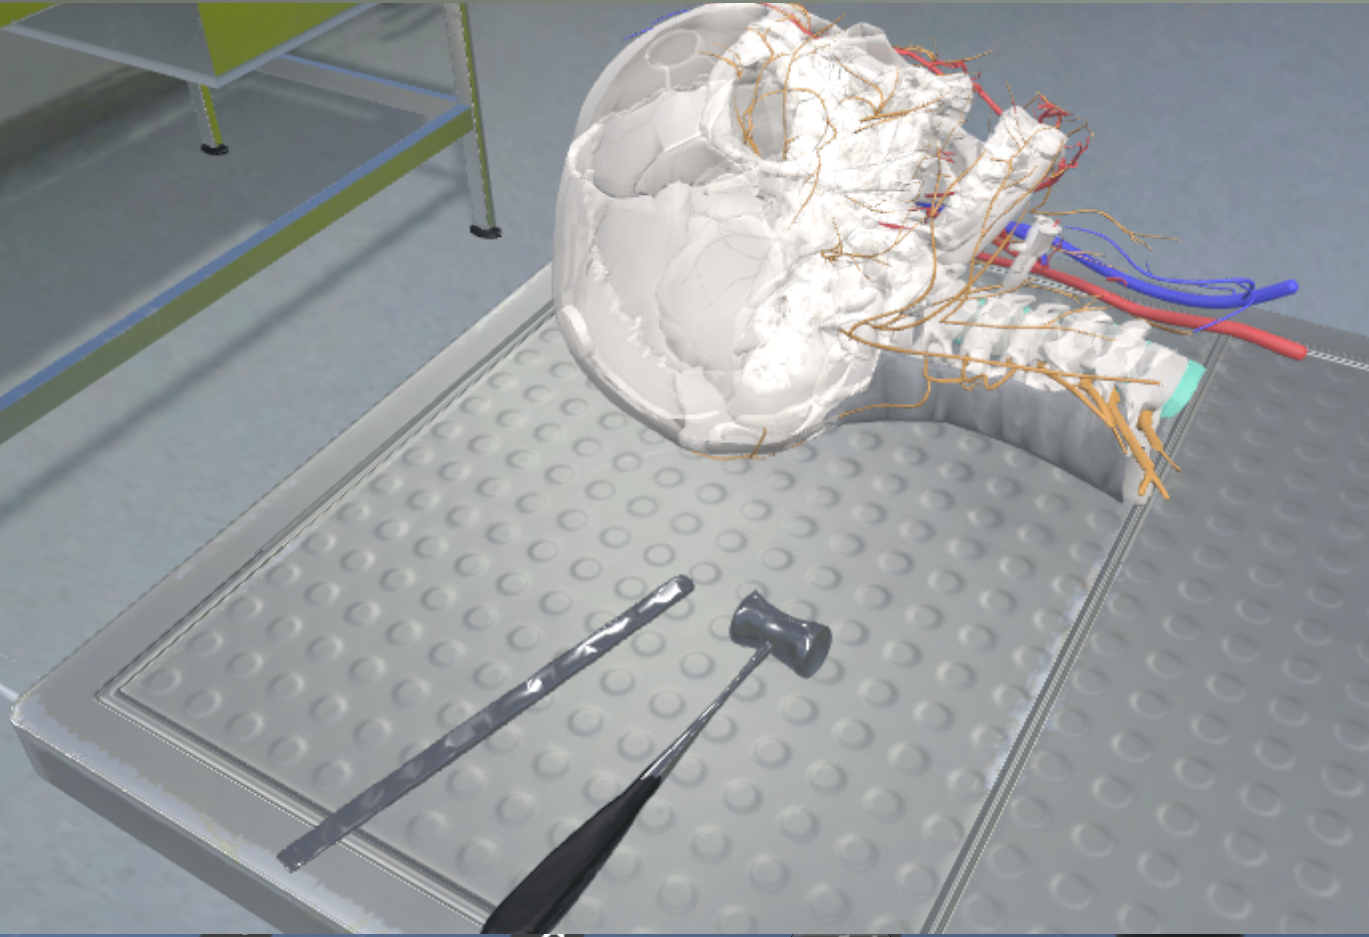
\includegraphics[width=\linewidth]{images/implementation/features/procedures/chisel_prepare.png}
    \caption{\label{fig::ChiselPrepare}The user prepares for the chiseling procedure by placing the instruments on the OT where the patient is located.
    indicators with the hammer in the other hand to perform the procedure.}
\end{figure}

When users have the perfect viewpoint, they can take up both instruments once again and start the procedure.
By pressing the indicate button on the hand where the chisel is located, rectangular indications at the top and bottom end of the chisel are shown to the user.
While these indications are active, the user has to perform a hammering motion with the hand holding the hammer.

\begin{figure}[ht]
    \centering
    \begin{minipage}{.5\textwidth}
      \centering
      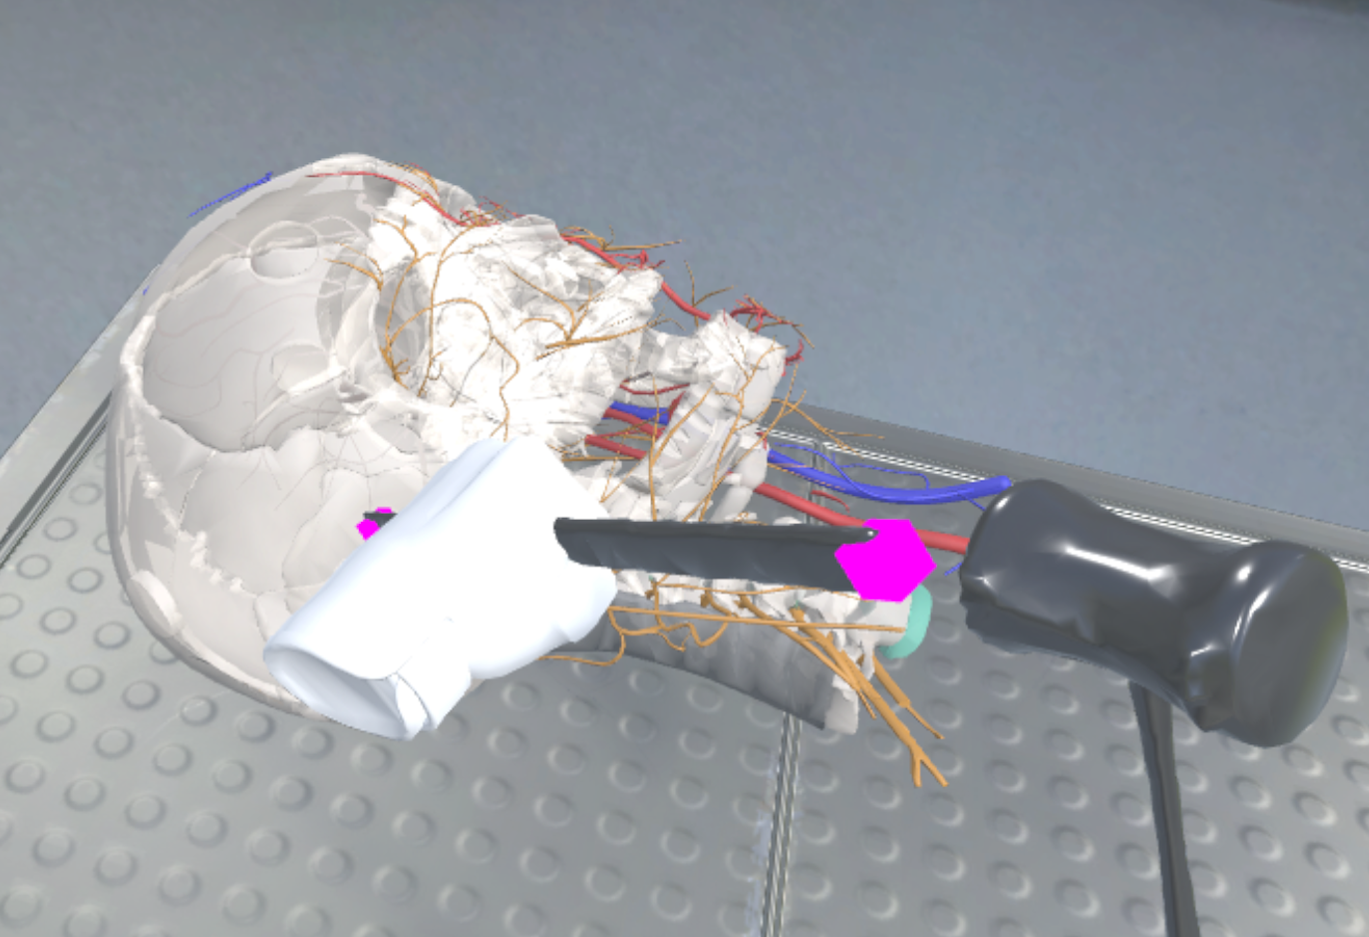
\includegraphics[width=0.99\linewidth]{images/implementation/features/procedures/chisel_1.png}
    \end{minipage}%
    \begin{minipage}{.5\textwidth}
      \centering
      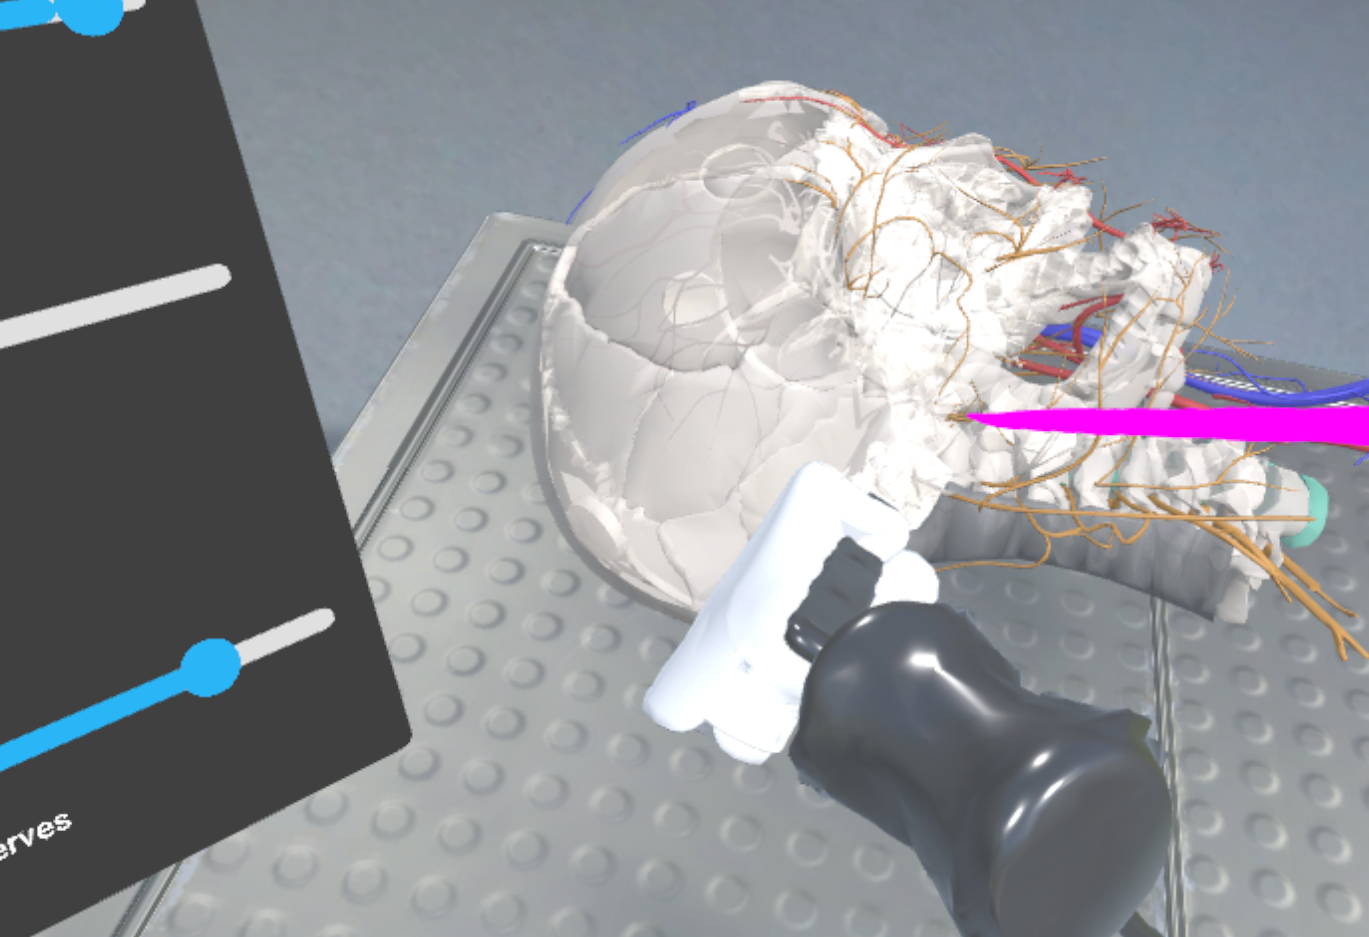
\includegraphics[width=0.99\linewidth]{images/implementation/features/procedures/chisel_2.png}
    \end{minipage}
    \caption{\label{fig::ChiselProcedure}Process of the chiseling procedure. Left: The users uses the indicate action with his left hand in preparation for the procedure. Right: After hammering on the indication on the chisel, the procedure has been performed and a step is generated.}
\end{figure}

When they hit the rectangular indicators located on the chisel, the chiseling procedure step is added to the project case in form of a modified copy of the hold chisel (Figure \ref{fig::ChiselProcedure}).
Here, information about the performed step is also included in the form of chisel size used for the procedure. 
\paragraph{Sawing}

\begin{figure}[ht]
    \centering
    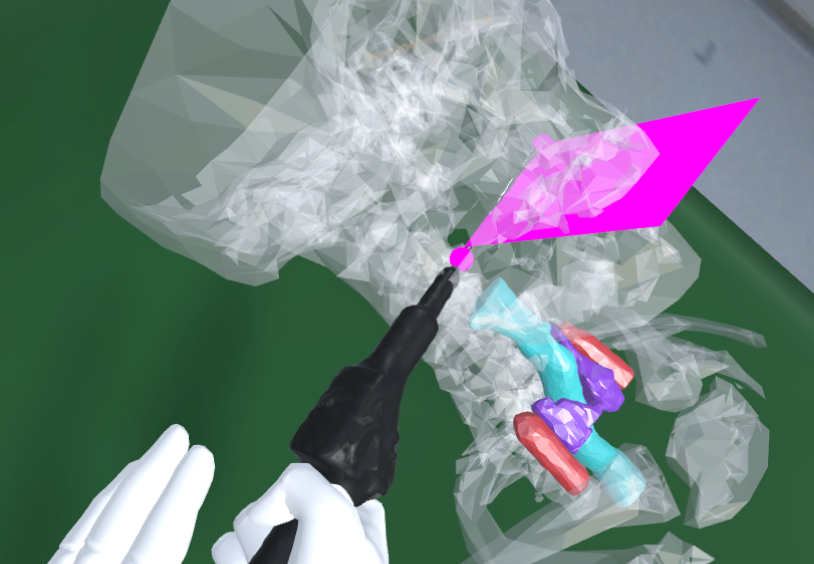
\includegraphics[width=200px]{images/implementation/features/procedures/bonesaw.png}
    \caption{\label{fig::FeatureBoneSaw}Bonesaw Procedure}
\end{figure}

The \textbf{sawing} procedure is performed by picking up the bonesaw.
Touch the controller will show two indications to the user (Figure \ref{fig::FeatureBoneSaw}).
The procedure is performed by first pressing down the trigger button and then letting go of it.
When letting go of the trigger button, a two dimensianal plane is created in the three dimensional space by using four points.
Two of these points are created when pressing down, and the other two when letting go of the trigger button.
A plane is then created with which the user can reproduce the way in which the bonesaw has been moved.
Arbitrary cutting shapes can be created by breaking them down into two-dimensional shapes and performing multiple movements.
\paragraph{Milling}

\begin{figure}[ht]
    \centering
    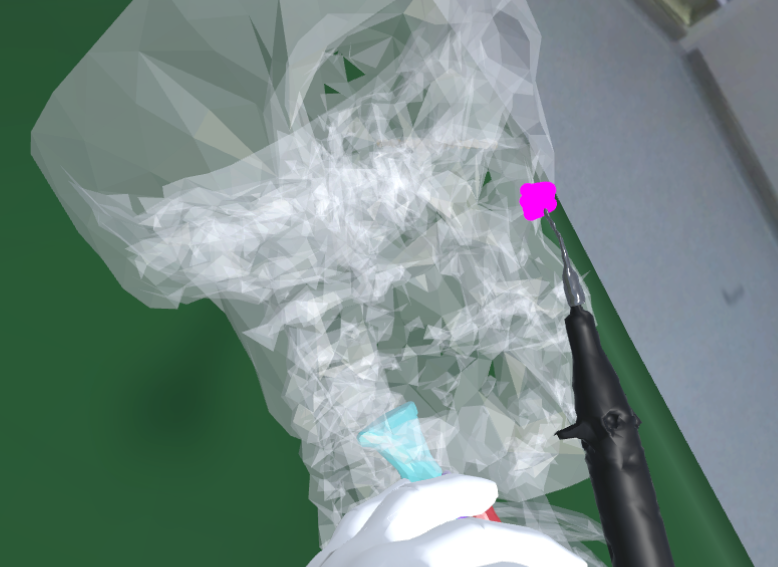
\includegraphics[width=200px]{images/implementation/features/procedures/piezo.png}
    \caption{\label{fig::FeaturePiezo}Milling procedure. Holding down the trigger button will draw little spheres until the button is released. The resulting object represents the volumetric space which is to be milled.}
\end{figure}

The \textbf{milling} operation is performed by grabbing the piezo instrument.
The indicator for the piezo is at the tip of the instrument, indicating which area will be milled.
While the "perform" button is being held down, little spheres are being drawn at the tip of the instrument \ref{fig::FeaturePiezo}.
When the button is released, the shapes are combined into a single 3D model and added as a project step.
The resulting object represents the volumetric space which has to be milled in the procedure.
The procedure can be reconstructed by "milling" the same 3D space in the virtual operating room.
\begin{figure}[ht!]
    \centering
    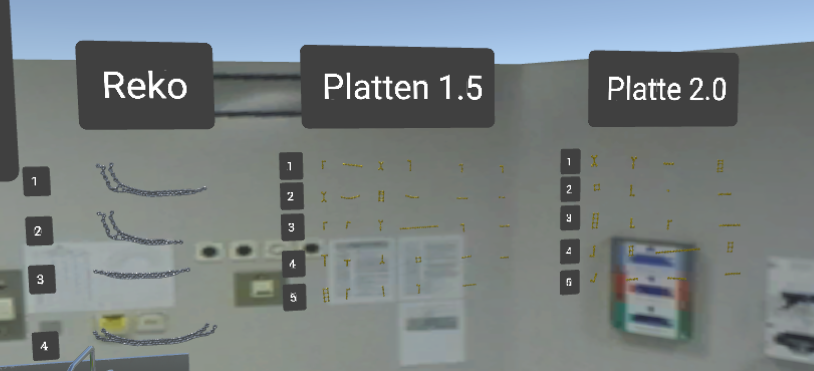
\includegraphics[width=\linewidth]{images/implementation/features/procedures/metal_plates_1.png}
    \caption{\label{fig::FeatureMetalPlate} Osteosynthesis Plates Overview}
\end{figure}

The osteosynthesis plates procedure consists of two steps before adding it as a step to the project case.
First, users have to chose which plate to use (Figure \ref{fig::FeatureMetalPlate}).
The user can chose from four reconstruction plates, 29 1.5mm plates and 20 2.0mm plates (Firma Angeben, osteosynthesis plates).
The optimal plates to use vary due to the pathology of the patient and the previously performed procedures.
After selecting the proper plate, a number of indicators will show to the user (Figure \ref{fig::FeatureMetalPlate2}).
In the context of the osteosynthesis plates, these indicators are "control points", with which the user can bend and twist the plates.
Bending and twisting is performed by chosing a control point via hovering them with the users free hand and grabbing them.
Then, the user has to translate and rotate the control point in the desired manner.
\begin{figure}
  \centering
  \begin{minipage}{.5\textwidth}
    \centering
    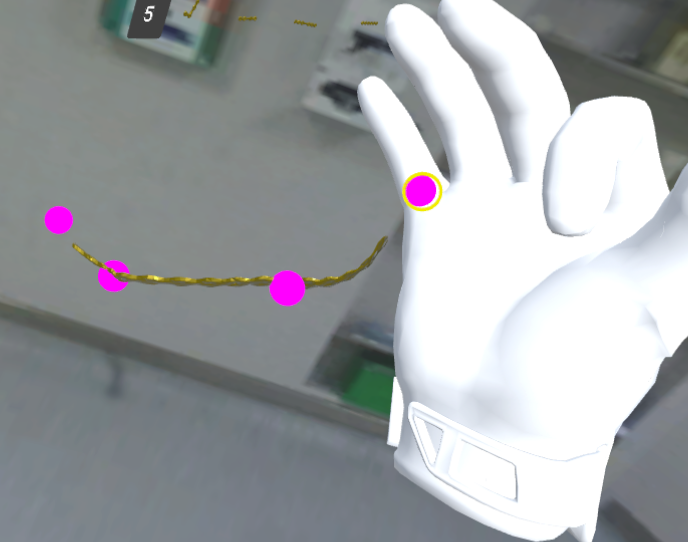
\includegraphics[width=0.95\linewidth]{images/implementation/features/procedures/metal_plates_2.png}
  \end{minipage}%
  \begin{minipage}{.5\textwidth}
    \centering
    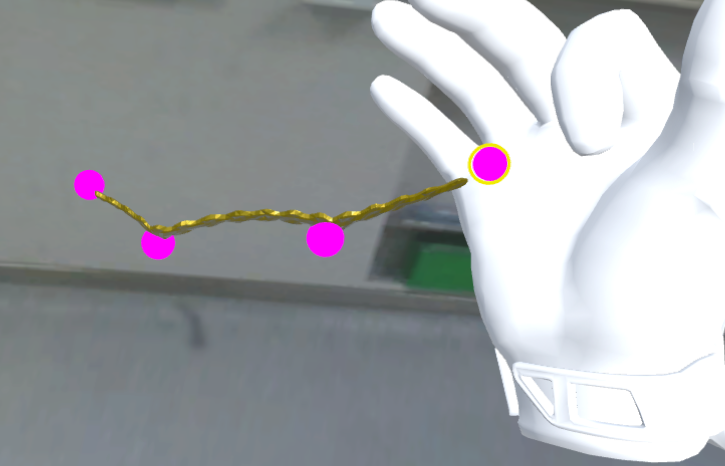
\includegraphics[width=0.95\linewidth]{images/implementation/features/procedures/metal_plates_3.png}
  \end{minipage}
  \caption{\label{fig::FeatureMetalPlate2}Osteosynthesis Plates Modifications. User can translate and rotate "control points" to perform modifications to the plates shape} 
\end{figure}

The user can then observe in which way this has affected the shape of the metal plate and either position the plate on the patient or perform more modifications to the plates via controlpoints.
The correct modification of the metal plates differs quite a lot from real life modifications to the plates.
However even though there is a slight learning curve to it, the modification is consistent and predictable (Figure \ref{fig::FeatureMetalPlate2}).


\begin{figure}[ht!]
    \centering
    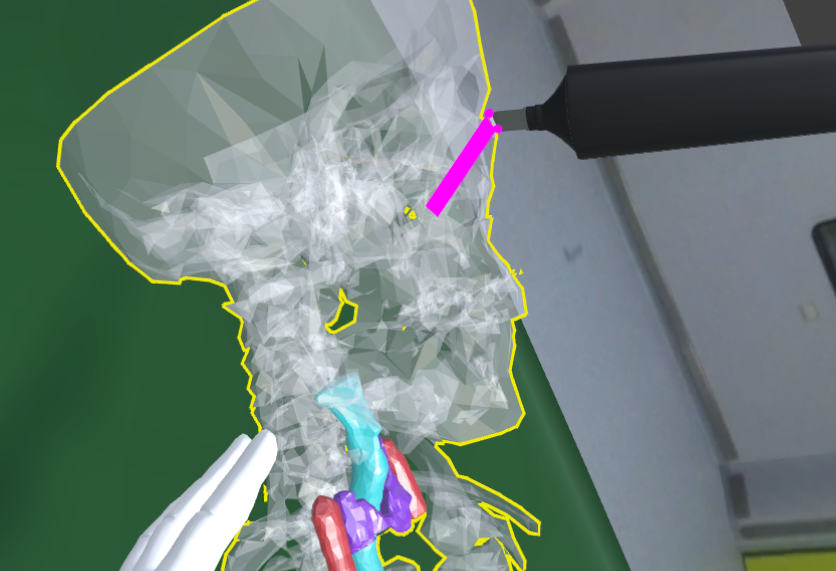
\includegraphics[width=\linewidth]{images/implementation/features/procedures/marker.png}
    \caption{\label{fig::FeatureMarker}Marker Procedure}
\end{figure}

The marking procedure is similar to the bonesaw procedure, meaning that rectangular shapes are drawed into the three dimensianal space (Figure \ref{fig::FeatureMarker}).
However, here the created shapes are much thinner.
In contrast to the bonesaw, the virtual hands of the user are also disabled here.
This way, the user can decide to hold the marker in the optimal way.
Since the main objective is marking specific spots on the patient, this is the natural approach.